\documentclass{article}
\usepackage{fancyhdr}
\usepackage{ctex}
\usepackage{listings}
\usepackage{graphicx}
\usepackage[a4paper, body={18cm,22cm}]{geometry}
\usepackage{amsmath,amssymb,amstext,wasysym,enumerate,graphicx}
\usepackage{float,abstract,booktabs,indentfirst,amsmath}
\usepackage{array}
\usepackage{booktabs}
\usepackage{multirow}
\usepackage{url}
\usepackage{diagbox}
\renewcommand\arraystretch{1.4}
\usepackage{indentfirst}
\setlength{\parindent}{2em}
\usepackage{enumitem}
\setmonofont{Consolas}
\usepackage{listings}
\usepackage{xcolor}
\usepackage{makecell}
\usepackage{tikz}
\usetikzlibrary{positioning, arrows.meta}
\setCJKmonofont{黑体}
\lstset{  
	% 基本设置  
	xleftmargin = 3em, xrightmargin = 3em, aboveskip = 1em,  
	backgroundcolor = \color{white},  
	basicstyle = \small\ttfamily,  
	rulesepcolor = \color{gray},  
	breaklines = true,  
	numbers = left,  
	numberstyle = \small,  
	numbersep = -14pt,  
	frame = shadowbox,  
	showspaces = false,  
	columns = fixed,  
	sensitive = true,  
	% VSCode 风格配色  
	keywordstyle = \color{blue!70!black}\bfseries,  
	emphstyle = \color{red!70!black}\bfseries, % 对于强调的词  
	emphstyle=[2]\color{purple!70!black}\bfseries, % 对于第二组强调的词  
	commentstyle = \color{green!60!black}, % 注释颜色  
	stringstyle = \color{orange!90!black}, % 字符串颜色更亮一些  
	morekeywords={ASSERT, int64\_t, uint32\_t},  
	moreemph={ASSERT, NULL},  
	moreemph=[2]{int64\_t, uint32\_t, tid\_t, uint8\_t, int16\_t, uint16\_t, int32\_t, size\_t, bool},  
	morecomment=[l][\color{green!60!black}]{+}, % 以+开头的注释  
}

%--------------------页眉--------------------%
\pagestyle{fancy}
\fancyhead[L]{}
\fancyhead[R]{}
\fancyhead[C]{华东师范大学软件工程学院实验报告}
\fancyfoot[C]{-\thepage-}
\renewcommand{\headrulewidth}{1.5pt}
%--------------------标题--------------------%
\begin{document}
\begin{center}
	{\Large{\textbf{\heiti 实验五——参数传递与系统调用}}}
	\begin{table}[H]
		\centering
		\begin{tabular}{p{2cm}p{4cm}<{\centering}p{1cm}p{2cm}p{6cm}<{\centering}}
			课程名称:    & 操作系统实践 & \quad & 指导教师:    & 张民
			\\ \cline{2-2} \cline{5-5}
			姓\qquad 名: & 王海生    & \quad & 学\qquad 号: & 10235101559         \\ \cline{2-2} \cline{5-5}
			实验编号:    & 实验五 & \quad & 实验名称:    & 参数传递与系统调用
			\\ \cline{2-2} \cline{5-5}
		\end{tabular}
	\end{table}
	
	% 添加新行并居中
	%\vspace{1em} % 可选:添加垂直间距
	\textbf{代码仓库:}\url{https://github.com/Hanson-Wang-chn/ECNU-Operating-System-WHS.git}
\end{center}
\rule{\textwidth}{1pt}

\tableofcontents

%--------------------正文--------------------%
\section{实验目的}

\begin{enumerate}
	\item 完成参数传递和部分系统调用(\texttt{exit}和\texttt{write}),使得\texttt{make check}通过\texttt{args}相关的5个测试。
	\item 完成实验报告并提交。
\end{enumerate}

\normalsize

\section{实验内容与设计思想}

\subsection{参数传递}

\begin{enumerate}
	\item 
	\textbf{字符串解析:}
	
	为了准确地获取启动新进程所需的各项信息,首先需要对传入的命令行字符串进行解析。这里采用了strtok\_r函数来分离进程名称和其他参数,同时为了避免直接修改原始字符串,我们在处理前对其进行了复制。
	
	\item 
	\textbf{内存管理:}
	
	考虑到性能和安全性,所有临时使用的数据结构都应在适当的时候释放。例如,在提取进程名后立即将不再需要的副本释放;而在加载程序失败的情况下,则立即清理已分配但未使用的资源。
	
	\item
	\textbf{栈布局调整:}
	
	为了让新创建的进程能够接收到正确的参数列表,我们需要按照特定格式将参数压入栈中。这涉及到更新\texttt{intr\_frame}结构体中的指针,确保当模拟返回中断时,新进程可以访问到完整的环境设置。
\end{enumerate}

\subsection{系统调用}

\begin{enumerate}
	\item 
	\textbf{注册机制:}
	
	为了支持新的系统调用,必须先定义它们的编号,并为每个调用关联一个处理函数。通过建立一个数组来存储这些处理函数的地址,我们可以根据调用号快速定位到对应的处理器。
	
	\item 
	\textbf{实现方法:}
	
	\begin{itemize}
		\item 对于\texttt{exit}系统调用,实现了向内核报告退出状态的功能,允许子进程结束时给父进程反馈结果。
		\item \texttt{write}系统调用负责处理标准输出流的数据写入操作,它会检查文件描述符是否合法,并将缓冲区的内容打印出来。
		\item \texttt{wait}系统调用用于等待某个子进程终止,并获取它的退出代码。为此,我们设计了一个\texttt{exit\_info}结构来跟踪子进程的状态,并利用信号量解决了父子进程间的同步问题。
	\end{itemize}
\end{enumerate}

\section{使用环境}

\subsection{主机系统配置}

本次实验的主机系统环境如下表所示:

\begin{center}
	\begin{tabular}{| >{\centering\arraybackslash}m{3cm} | >{\centering\arraybackslash}m{7cm} |}    
		\hline  
		\textbf{项目名称} & \textbf{详细信息} \\
		\hline  
		操作系统 & macOS Sequoia 15.2 \\  
		\hline  
		系统类型 & 64位操作系统,基于ARM的处理器 \\  
		\hline
		CPU & Apple M1 Pro \\  
		\hline 
		GPU & Apple M1 Pro\\  
		\hline 
		内存 & 32GB 统一内存 \\  
		\hline 
		磁盘 & 512GB SSD \\  
		\hline 		
	\end{tabular}
\end{center}

\subsection{Docker配置}

在官网下载并安装后,Docker容器正常运行,如下图所示:

\begin{figure}[H]
	\centering
	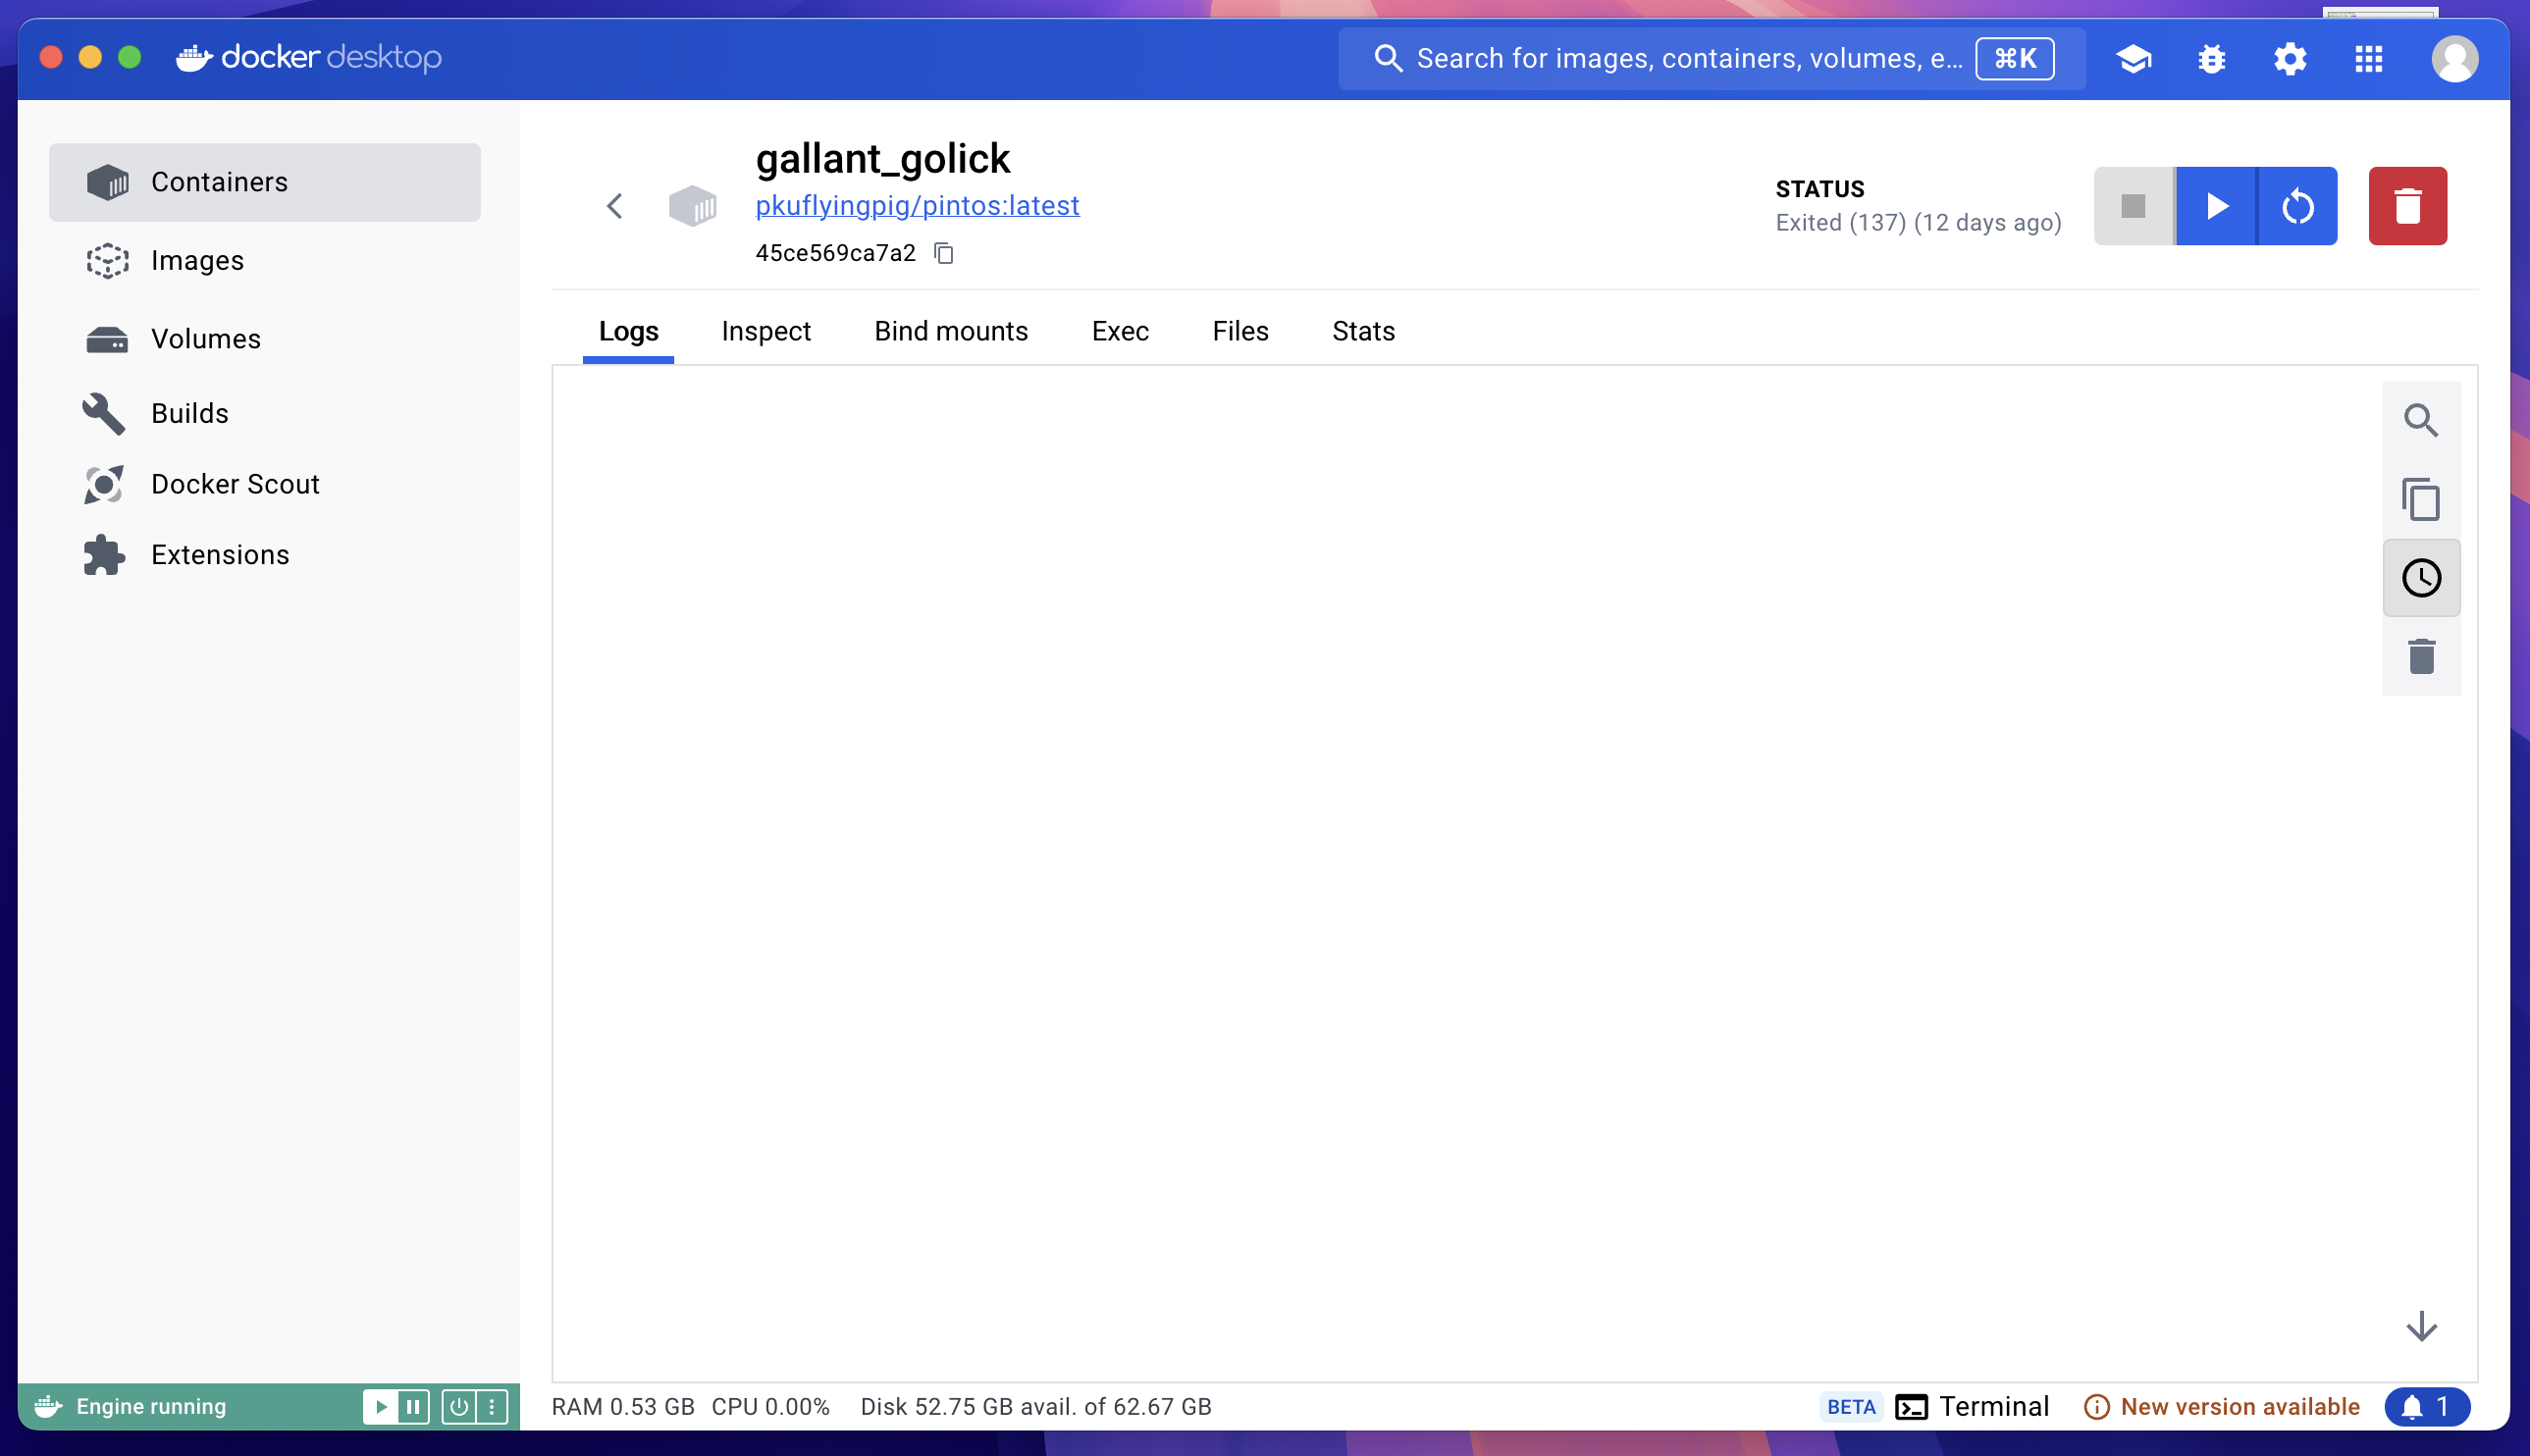
\includegraphics[width=0.9\textwidth]{img/docker_install.png}
	\caption{Docker容器}
\end{figure}

接着使用下面的命令实现磁盘挂载,方便文件管理:

\begin{lstlisting}[language=Bash, title=启动Docker容器并挂载文件]
	docker run -it --rm --name pintos --mount type=bind,source=/Users/wanghaisheng/Desktop/Coding/Courses/ECNU-Operating-System-WHS/pintos,target=/home/PKUOS/pintos pkuflyingpig/pintos bash
\end{lstlisting}

完成后如下图所示:

\begin{figure}[H]
	\centering
	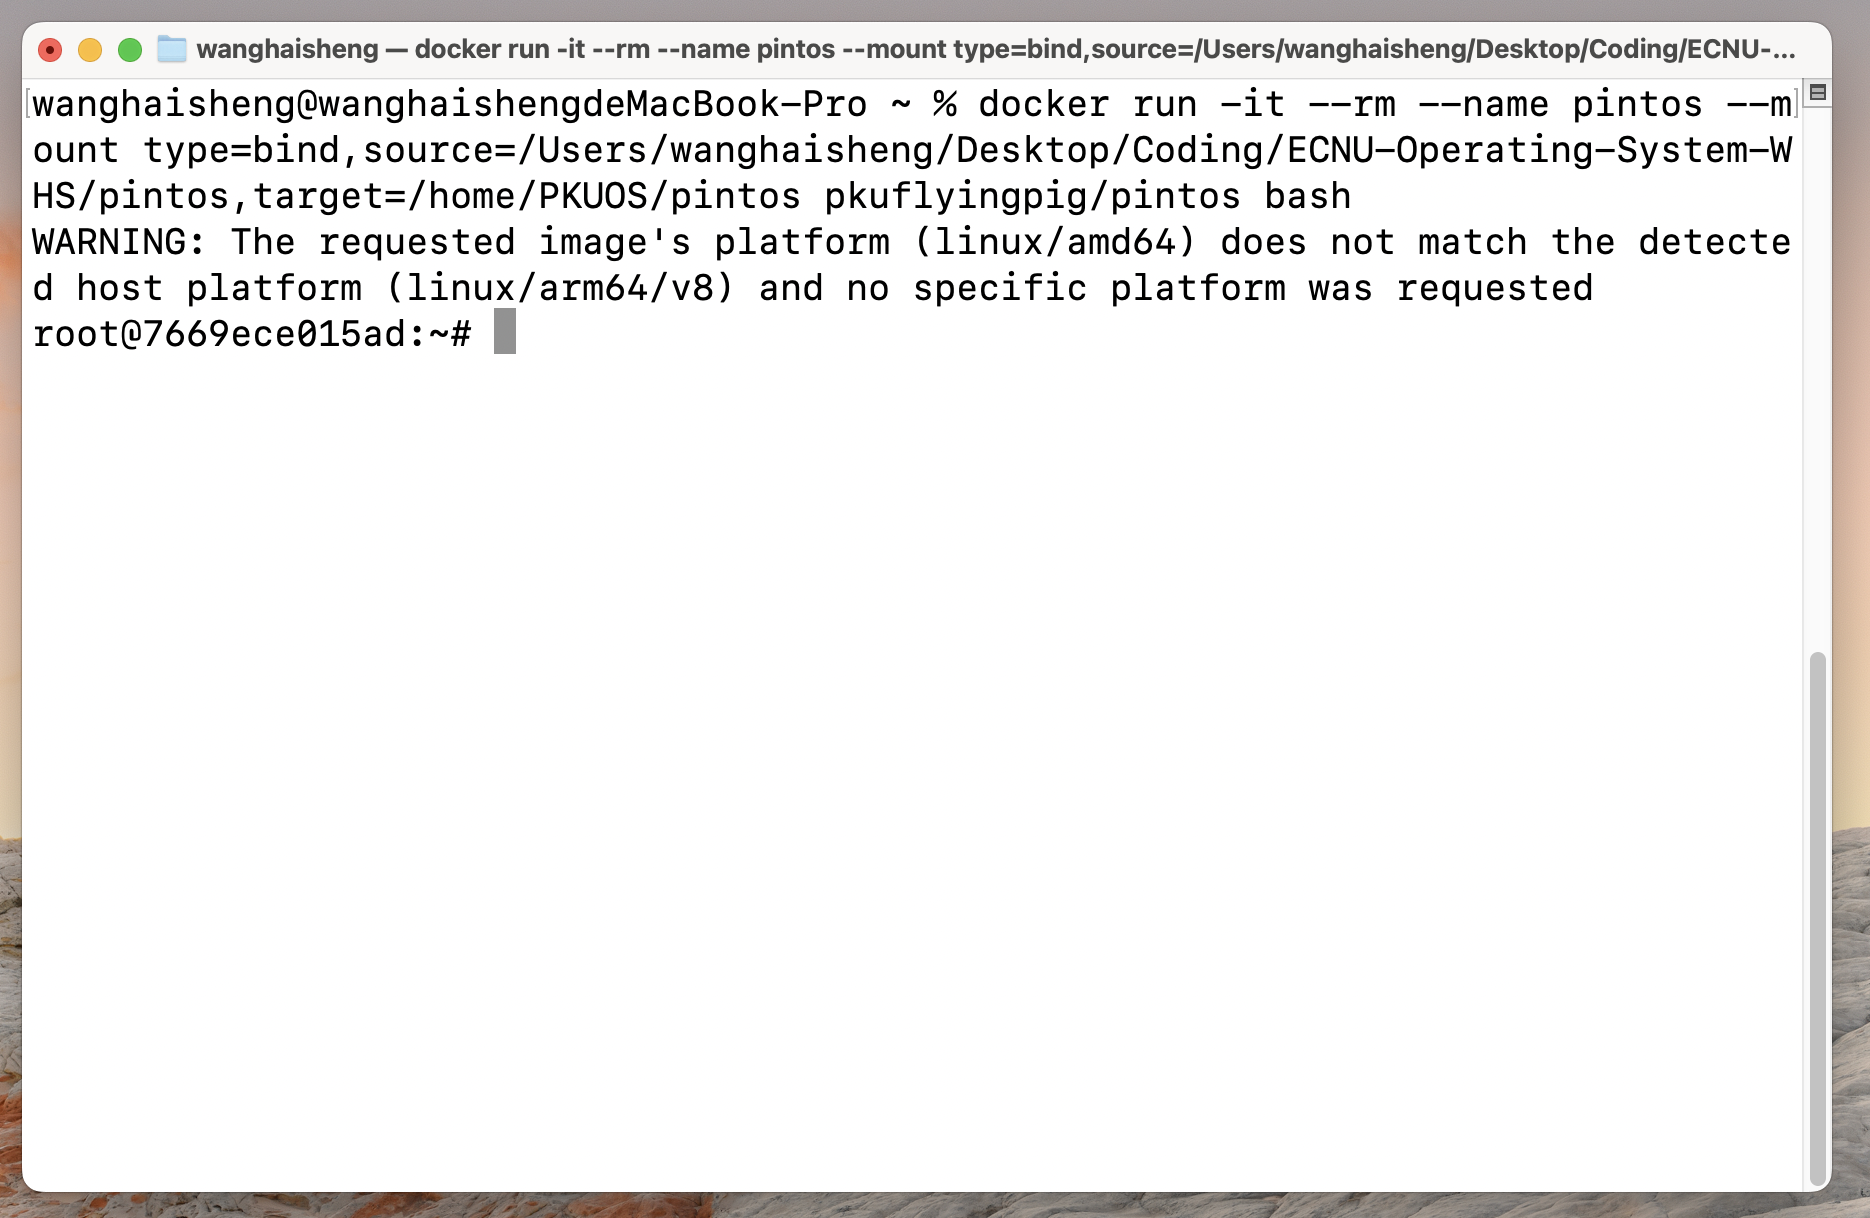
\includegraphics[width=0.9\textwidth]{img/run_docker.png}
	\caption{完成环境配置}
\end{figure}

\section{Argument Passing}

参数分离的任务是从传入的命令字符串中解析出文件名和文件参数,因此需要对输入的字符串进行分割。在审查 \texttt{process\_execute} 函数的过程中发现,此函数调用 \texttt{thread\_create} 时,第一个参数代表进程的名字,而最后一个参数则是用户提供的完整字符串。

首先,应提取输入字符串的第一个子串作为进程的名字(这虽然有助于调试,但并非强制要求;也可以选择任意名称)。根据提示,采用 \texttt{strtok\_r} 函数来实现这一操作。通过查阅该函数的文档得知,\texttt{strtok\_r} 在处理过程中会修改原始字符串,所以应该在分割进程名称之前复制一份新的字符串以确保原始字符串保持不变。

遵循 \texttt{process\_execute} 中的内存分配策略,为新复制的字符串分配一个页面大小的空间。考虑到该字符串的使用周期,它将在 \texttt{init\_thread} 中被复制到进程信息结构体中,由此可以确定,在 \texttt{thread\_create} 调用之后,该字符串将不再有其他用途,因此应在函数结束前释放该页空间。

对于 \texttt{fn\_copy} 的生命周期管理:如果进程创建失败,则应立即释放该页;若进程创建成功,\texttt{fn\_copy} 的所有权将转移给新进程负责,这意味着 \texttt{file\_name} 将在 \texttt{start\_process} 中得到适当的释放。

\begin{lstlisting}[language=C]
	tid_t process_execute(const char* file_name) { 
		char* fn_copy, *name_copy; tid_t tid;
		fn_copy = palloc_get_page(0); 
		name_copy = palloc_get_page(0); 
		if(fn_copy == NULL || name_copy == NULL) return TID_ERROR;
		strlcpy(fn_copy, file_name, PGSIZE); 
		strlcpy(name_copy, file_name, PGSIZE);
		char* save_ptr; 
		name_copy = strtok_r(name_copy,"",&save_ptr);
		tid = thread_create(name_copy, PRI_DEFAULT, start_process, fn_copy);
		palloc_free_page(name_copy);
		if(tid == TID_ERROR) palloc_free_page(fn_copy);
		return tid; 
	}
\end{lstlisting}

根据实验手册,进程创建的最后一步是推送一个虚拟的返回地址,具体是在 \texttt{start\_process} 中通过内联汇编语句 \texttt{asm volatile("movl \%0, \%\%esp; jmp intr\_exit"::"g"(\&if\_):"memory");} 来实现。在此之前,需要将所有参数压入栈中,并更新 \texttt{intr\_frame} 结构体。

前面提到,进程的名字不一定等同于要加载的程序名称,因此在这里需要再次复制字符串以获取实际要加载的程序名。同时需要注意的是,原始对象的生命周期在 \texttt{load} 函数执行完毕后即告终止,因此应确保释放这些资源。

在 \texttt{load} 操作完成后,实现了名为 \texttt{push\_arguments} 的函数用于将参数压入栈中。该函数确保了在设置虚假返回地址之前,所有必要的参数已经被正确地放置在栈上,准备就绪以供新进程使用。

\begin{lstlisting}[language=C]
	void push_argument(void** esp, char* cmd) { 
		int argc = 0, argv[64]; 
		char* token, *save_ptr;
		(*esp) = PHYS_BASE;
		for(token = strtok_r(cmd," ",&save_ptr); token != NULL; token = strtok_r(NULL," ",&save_ptr)) { 
			size_t len = strlen(token); 
			(*esp) -= (len + 1); 
			memcpy((*esp), token, len + 1); 
			argv[argc++] = (*esp); 
		}
		(*esp) = (int)(*esp) & 0xfffffffc; // word_align 
		(*esp) -= 4, (*(int*)(*esp)) = 0; // argv[argc]
		for(int i = argc - 1; i >= 0; i--)// argv[i]; 
		(*esp) -= 4, (*(int*)(*esp)) = argv[i];
		(*esp) -= 4, (*(int*)(*esp)) = (*esp) + 4;// argv 
		(*esp) -= 4, (*(int*)(*esp)) = argc; // argc
		(*esp) -= 4, (*(int*)(*esp)) = 0; // return address 
	}
\end{lstlisting}

新复制的字符串同样需要严格管理其生命周期。如果 \texttt{load} 操作失败,则必须释放该字符串并终止进程,以避免内存泄漏;反之,若 \texttt{load} 成功执行,在将参数压入栈中之后应立即释放该字符串,确保资源得到妥善处理。

由于测试输出现在是通过系统调用来实现的(这与 Project 1 中直接打印的方式有所不同),当前使用 \texttt{make check} 进行测试将会导致所有测试结果都显示为失败。然而,根据手册指导,可以利用 \texttt{hex\_dump} 函数来打印栈上的值,以此作为调试和验证的一种手段。

\begin{lstlisting}[language=C]
	static void start_process(void* file_name_) { 
		char* file_name = file_name_; 
		struct intr_frame if_; 
		bool success;
		/* Initialize interrupt frame and load executable.*/ 
		memset(&if_, 0, sizeof if_); 
		if_.gs = if_.fs = if_.es = if_.ds = if_.ss = SEL_UDSEG; 
		if_.cs = SEL_UCSEG; 
		if_.eflags = FLAG_IF | FLAG_MBS;
		char* cmd = palloc_get_page(0); 
		strlcpy(cmd, file_name_, PGSIZE);
		char* save_ptr; 
		file_name = strtok_r(file_name," ",&save_ptr); 
		success = load(file_name,&if_.eip,&if_.esp); 
		palloc_free_page(file_name);
		if(!success) { 
			palloc_free_page(cmd); 
			thread_exit(); 
		}
		push_argument(&if_.esp, cmd); 
		hex_dump((uintptr_t)if_.esp, if_.esp,(PHYS_BASE) - if_.esp, true); 
		palloc_free_page(cmd);
		/* Start the user process by simulating a return from an interrupt, implemented by intr_exit(in threads/intr-stubs.S).  Because intr_exit takes all of its arguments on the stack in the form of a`struct intr_frame', we just point the stack pointer(%esp) to our stack frame and jump to it.*/
		asm volatile("movl %0,%%esp; jmp intr_exit"::"g"(&if_):"memory"); 
		NOT_REACHED(); 
	}
\end{lstlisting}

执行 \texttt{make \&\& pintos --filesys-size=2 -p tests/userprog/args-multiple-a args-multiple-- -f extract run 'args-multiple some arguments for you!'} 后 \texttt{hex\_dump} 的结果如下:

\begin{lstlisting}
	bfffffb0 00 00 00 00-05 00 00 00 c0 ff ff bf| ............|
	bfffffc0 f2 ff ff bf ed ff ff bf-e3 ff ff bf df ff ff bf|................|
	bfffffd0 da ff ff bf 00 00 00 00-00 00 79 6f 75 21 00 66|..........you!.f|
	bfffffe0 6f 72 00 61 72 67 75 6d-65 6e 74 73 00 73 6f 6d|or.arguments.som| 
	bffffff0 65 00 61 72 67 73 2d 6d-75 6c 74 69 70 6c 65 00|e.args-multiple.|
\end{lstlisting}

\section{System Call}

\subsection{注册系统调用}

系统调用号在 \texttt{lib/syscall-nr.h} 中定义。根据文档,系统调用号会被放置在栈顶,随后的参数则依次压入栈中。为了简化函数调用的过程,这里采用一个数组来存储各函数的地址。具体而言,在注册系统调用时,使用对应的系统调用号作为数组的下标,将相应的 handler 函数地址存储到该位置。这样一来,在处理系统调用时,只需要从栈中取出系统调用编号,并据此调用相应的函数即可。

这种方法不仅提高了查找效率,还使得代码结构更加清晰简洁,便于维护和扩展。

\begin{lstlisting}[language=C]
	void syscall_halt(struct intr_frame* f) { } 
	void syscall_exit(struct intr_frame* f) { } 
	void syscall_exec(struct intr_frame* f) { } 
	void syscall_wait(struct intr_frame* f) { } 
	void syscall_create(struct intr_frame* f) { } 
	void syscall_remove(struct intr_frame* f) { } 
	void syscall_open(struct intr_frame* f) { } 
	void syscall_filesize(struct intr_frame* f) { } 
	void syscall_read(struct intr_frame* f) { } 
	void syscall_write(struct intr_frame* f) {
	} 
	void syscall_seek(struct intr_frame* f) { } 
	void syscall_tell(struct intr_frame* f) { } 
	void syscall_close(struct intr_frame* f) { }
\end{lstlisting}

\begin{lstlisting}[language=C]
	int (*func[20])(struct intr_frame*);
\end{lstlisting}

\begin{lstlisting}[language=C]
	void syscall_init(void) { 
		intr_register_int(0x30, 3, INTR_ON, syscall_handler,"syscall"); 
		func[SYS_HALT] = syscall_halt; 
		func[SYS_EXIT] = syscall_exit; 
		func[SYS_EXEC] = syscall_exec; 
		func[SYS_WAIT] = syscall_wait; 
		func[SYS_CREATE] = syscall_create; 
		func[SYS_REMOVE] = syscall_remove; 
		func[SYS_OPEN] = syscall_open; 
		func[SYS_FILESIZE] = syscall_filesize; 
		func[SYS_READ] = syscall_read; 
		func[SYS_WRITE] = syscall_write; 
		func[SYS_SEEK] = syscall_seek; 
		func[SYS_TELL] = syscall_tell; 
		func[SYS_CLOSE] = syscall_close; 
	}
\end{lstlisting}

\begin{lstlisting}[language=C]
	static void syscall_handler(struct intr_frame* f UNUSED) { 
		int number = *(int*)(f->esp); 
		(func[number])(f); 
	}
\end{lstlisting}

\subsection{实现系统调用}

为了支持参数传递(Argument Passing)的测试,这里采用较为简单的方法来实现\texttt{SystemCall}。

\subsubsection{exit}

根据函数声明 \texttt{void exit(int status)}: 该函数用于终止当前进程,并向内核返回一个表示退出状态的错误码。为了终止当前进程,只能调用 \texttt{thread\_exit} 函数,而 \texttt{thread\_exit} 内部则会进一步调用 \texttt{process\_exit} 函数。为了确保线程安全地将错误码返回给内核,可以将错误码存储在 \texttt{thread} 结构体中。请注意,在 \texttt{init\_thread} 函数中应当初始化 \texttt{t->error\_code = 0}。

通过全局搜索 \texttt{thread\_exit} 可知,在任何异常退出的情况下都应设置错误码。例如,在文件 \texttt{exception.c} 中的 \texttt{kill} 函数里,应设置 \texttt{thread\_current()->exit\_code = -1};同样地,在刚刚实现的 \texttt{start\_process} 函数中也需进行相应的设置。为此,可以定义以下辅助函数来简化这一过程。

\begin{lstlisting}[language=C]
	// thread.c 
	void error_exit() { 
		thread_current()->exit_code = -1; 
		thread_exit(); 
	}
\end{lstlisting}

在系统调用中同样按照参数位置设置错误码并终止进程。

\begin{lstlisting}[language=C]
	void syscall_exit(struct intr_frame* f) { 
		int exit_code = *(int*)(f->esp + 4); 
		thread_current()->exit_code = exit_code; 
		thread_exit(); 
	}
\end{lstlisting}

\subsubsection{write}
首先就是根据函数声明 \texttt{int write(int fd, const void* buffer, unsigned size)} 来获取参数。
fd 是文件描述符,当 \texttt{fd == 0} 时是标准输入流,不是 write操作,所以直接退出,当 \texttt{fd == 1} 时是标 准输出流,需要把内容写到缓冲区,本报告只实现写入缓冲区的功能。

尽管实现了上述功能,测试仍然未能通过,问题在于主进程在子进程结束之前就已经退出了。为了确保主进程正确地等待子进程完成其任务,必须在主进程中添加相应的逻辑来同步子进程的生命周期,例如使用等待(wait)系统调用来确保主进程不会提前退出。

\begin{lstlisting}[language=C]
	void syscall_write(struct intr_frame* f) { 
		int fd = *(int*)(f->esp + 4); 
		char* buf = *(char**)(f->esp + 8); 
		int size = *(int*)(f->esp + 12);
		if(fd == 0) error_exit();
		if(fd == 1) { 
			putbuf(buf, size); 
			f->eax = size; 
		} 
	}
\end{lstlisting}

\subsubsection{wait}

根据函数声明 \texttt{int wait(pid\_t pid)},该函数的作用是依据传入的子进程 \texttt{pid} 来获取并返回其退出状态码。为了确保在子进程退出后仍能访问到它的相关信息,解决方案是在每个进程中创建一个名为 \texttt{exit\_info} 的结构体,用于存储该进程的相关信息。具体来说,每个父进程会维护一个 \texttt{exit\_info} 列表,用来记录它所有的子进程的信息。此外,为了保证父进程和子进程之间的同步,将使用信号量(semaphore)来管理。

\texttt{exit\_info} 结构体应存储在堆上,并通过 \texttt{malloc} 分配内存。关于 \texttt{exit\_info} 的生命周期,它从进程创建时开始,直到没有任何进程需要这段信息为止——即当父进程结束时终止。因此,\texttt{exit\_info} 中还应该包含一个指向父进程的引用 \texttt{parent},以跟踪和管理其生命周期。这确保了在适当的时候可以正确地释放与子进程相关的资源,同时避免了内存泄漏问题。

\begin{lstlisting}[language=C]
	struct thread { 
		/* Owned by thread.c.*/
		tid_t tid; /**< Thread identifier.*/
		enum thread_status status; /**< Thread state.*/
		char name[16]; /**< Name(for debugging purposes).*/
		uint8_t* stack; /**< Saved stack pointer.*/
		int priority; /**< Priority.*/
		struct list_elem allelem; /**< List element for all threads list.*/
		struct list_elem waitelem; 
		int64_t wake_tick;
		/* Shared between thread.c and synch.c.*/
		struct list_elem elem; /**< List element.*/
		#ifdef USERPROG 
		/* Owned by userprog/process.c.*/
		uint32_t* pagedir; /**< Page directory.*/
		uint32_t exit_code;
		struct list child_list; 
		struct exit_info* linked_exit; 
		struct semaphore sema_wait;
		#endif
		/* Owned by thread.c.*/
		unsigned magic; /**< Detects stack overflow.*/
	};
	struct exit_info { 
		tid_t tid; 
		struct thread* linked_thread; 
		struct thread* parent; 
		int exit_code; 
		bool is_still_alive; 
		bool is_being_waited;
		struct list_elem child_elem; 
	};
\end{lstlisting}

在 \texttt{thread\_create} 和 \texttt{init\_thread} 中进行初始化。

\begin{lstlisting}[language=C]
	tid_t thread_create(const char* name, int priority, thread_func* function, void* aux) { 
		struct thread* t; 
		struct kernel_thread_frame* kf; 
		struct switch_entry_frame* ef; 
		struct switch_threads_frame* sf; 
		tid_t tid;
		ASSERT(function != NULL);
		/* Allocate thread.*/ 
		t = palloc_get_page(PAL_ZERO); 
		if(t == NULL) return TID_ERROR;
		/* Initialize thread.*/ 
		init_thread(t, name, priority); 
		tid = t->tid = allocate_tid();
		t->linked_exit = malloc(sizeof(struct exit_info)); 
		t->linked_exit->parent = thread_current(); 
		t->linked_exit->tid = tid; 
		t->linked_exit->linked_thread = t; 
		t->linked_exit->exit_code = 0; 
		t->linked_exit->tid = tid; 
		t->linked_exit->is_still_alive = true; 
		t->linked_exit->is_being_waited = false; 
		list_push_back(&t->linked_exit->parent->child_list,&t->linked_exit->child_elem);
		/* Stack frame for kernel_thread().*/ 
		kf = alloc_frame(t, sizeof*kf); 
		kf->eip = NULL; 
		kf->function = function; 
		kf->aux = aux;
		/* Stack frame for switch_entry().*/ 
		ef = alloc_frame(t, sizeof*ef);
		ef->eip = (void(*)(void)) kernel_thread;
		/* Stack frame for switch_threads().*/ 
		sf = alloc_frame(t, sizeof*sf); 
		sf->eip = switch_entry; 
		sf->ebp = 0;
		/* Add to run queue.*/ 
		thread_unblock(t); 
		thread_yield();
		return tid; 
	}
	static void init_thread(struct thread* t, const char* name, int priority) { 
		enum intr_level old_level;
		ASSERT(t != NULL); 
		ASSERT(PRI_MIN <= priority && priority <= PRI_MAX); 
		ASSERT(name != NULL);
		memset(t, 0, sizeof*t); 
		t->status = THREAD_BLOCKED; 
		strlcpy(t->name, name, sizeof t->name); 
		t->stack = (uint8_t*) t + PGSIZE; 
		t->priority = priority; 
		t->magic = THREAD_MAGIC; 
		t->wake_tick = -1;
		t->exit_code = 0; 
		list_init(&t->child_list); 
		sema_init(&t->sema_wait, 0);
		old_level = intr_disable();
		list_insert_ordered(&all_list,&t->allelem, thread_more_priority, NULL); 
		// list_push_back(&all_list,&t->allelem); 
		intr_set_level(old_level); 
	}
\end{lstlisting}

在系统调用中,只需调用 \texttt{process\_wait} 即可。根据文档描述,\texttt{process\_wait} 的功能是查找子进程;如果找到的子进程仍在运行,则执行 P 操作以使当前进程阻塞,直至子进程结束并获取其退出码。成功返回后,还需确保从相关链表中移除已等待的子进程记录。

相应地,每当有 P 操作存在时,必然伴随有 V 操作用于解除阻塞。具体到 \texttt{process\_exit} 函数中,它会遍历所有子进程来更新每个子进程的父进程引用 (\texttt{exit\_info->parent})。接着,该函数检查当前进程的退出信息 (\texttt{exit\_info}) 生命周期是否已经完成;若确实已完成,则进行资源释放。最后,更新或清理当前进程的退出信息字段。

\begin{lstlisting}[language=C]
	int process_wait(tid_t child_tid UNUSED) { 
		struct thread* cur = thread_current();
		struct list* l = &cur->child_list; 
		struct list_elem* e = NULL; 
		struct exit_info* child; 
		for(e = list_begin(l); e != list_end(l); e = list_next(e))
		{ 
			child = list_entry(e, struct exit_info, child_elem); 
			if(child->tid == child_tid) break; 
		}
		if(e == list_end(l)) return -1; 
		list_remove(e);
		if(child->is_still_alive) { 
			child->is_being_waited = true; 
			sema_down(&child->linked_thread->sema_wait); 
		}
		return child->exit_code; 
	}
	void process_exit(void) { 
		struct thread* cur = thread_current(); 
		uint32_t* pd;
		struct list* l = &cur->child_list; 
		struct list_elem* e; 
		for(e = list_begin(l); e != list_end(l); e = list_next(e)) { 
			struct exit_info* tmp = list_entry(e, struct exit_info, child_elem);
			if(tmp->is_still_alive) tmp->linked_thread->linked_exit->parent = NULL; 
		}
		if(cur->linked_exit->parent == NULL) free(cur->linked_exit); 
		else { 
			cur->linked_exit->exit_code = cur->exit_code; 
			if(cur->linked_exit->is_being_waited) sema_up(&cur->sema_wait);
			cur->linked_exit->is_still_alive = false; 
			cur->linked_exit->linked_thread = NULL; 
		}
		pd = cur->pagedir; 
		if(pd != NULL) { 
			cur->pagedir = NULL; 
			pagedir_activate(NULL); 
			pagedir_destroy(pd); 
		}
		printf("%s: exit(%d)\n", cur->name, cur->linked_exit->exit_code); 
	}
\end{lstlisting}

\texttt{wait} 的 \texttt{Syscall}只需要调用 \texttt{process\_wait} 函数即可。

\begin{lstlisting}[language=C]
	void syscall_wait(struct intr_frame* f) { 
		int pid = *(int*)(f->esp + 4); 
		f->eax = process_wait(pid); 
	}
\end{lstlisting}

至此可以通过\texttt{args}相关的测试点。

\begin{lstlisting}
	pass tests/userprog/args-none 
	pass tests/userprog/args-single 
	pass tests/userprog/args-multiple 
	pass tests/userprog/args-many 
	pass tests/userprog/args-dbl-space
\end{lstlisting}

至此,本实验相关的测试点全部通过.

\section{实验总结}

通过本次实验,我对操作系统中的参数传递和系统调用有了更深入的理解与掌握。在参数传递部分,学会了如何准确地解析命令行字符串,合理管理内存以及正确调整栈布局,这使我明白了进程创建过程中数据处理的重要性和复杂性。在系统调用方面,成功实现了\texttt{exit}、\texttt{write}和\texttt{wait}等系统调用,理解了系统调用的注册机制和实现方法,并且通过信号量解决了父子进程间的同步问题,这让我对操作系统的进程管理有了更清晰的认识。

\end{document}